\chapter{Participation statistics}

\section{Descriptives}

\begin{longtable}[c]{@{}lrrrrrrrrrr@{}}
\toprule\addlinespace
& N & min & max & mean & var & skew & kurt & normal-t & normal-p
\\\addlinespace
\midrule\endhead
\textbf{Flashcards} & 33 & 0 & 7 & 3.27 & 7.58 & 0.02 & -1.75 & 56.992 &
0.0000
\\\addlinespace
\textbf{Flashmap} & 30 & 0 & 11 & 3.27 & 10.41 & 0.39 & -1.04 & 3.868 &
0.1446
\\\addlinespace
\textbf{General} & 63 & 0 & 11 & 3.27 & 8.78 & 0.24 & -1.26 & 22.212 &
0.0000
\\\addlinespace
\bottomrule
    \label{tab:dropouts}
\end{longtable}

\begin{figure}
    \centering
    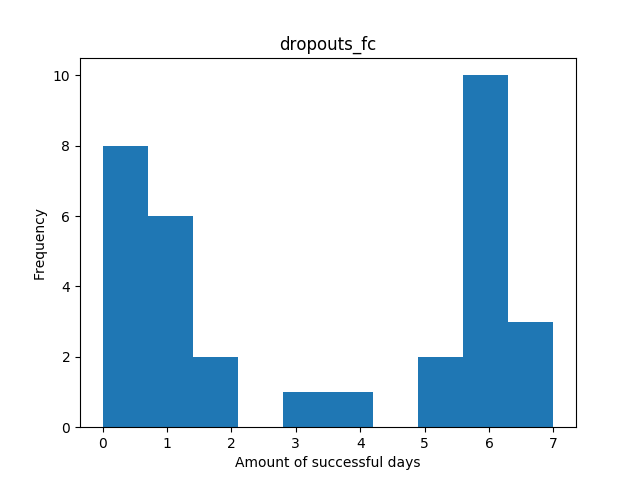
\includegraphics[width=.7\textwidth]{img/dropouts_fc.png}
    \caption{A histogram depicting the active days of the flashcard users}
    \label{fig:dropouts_fc}
\end{figure}
\begin{figure}
    \centering
    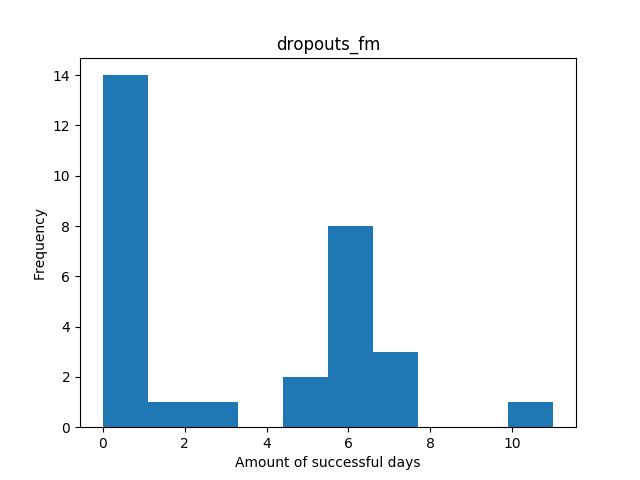
\includegraphics[width=.7\textwidth]{img/dropouts_fm.png}
    \caption{A histogram depicting the active days of the flashmap users}
    \label{fig:dropouts_fm}
\end{figure}
\begin{figure}
    \centering
    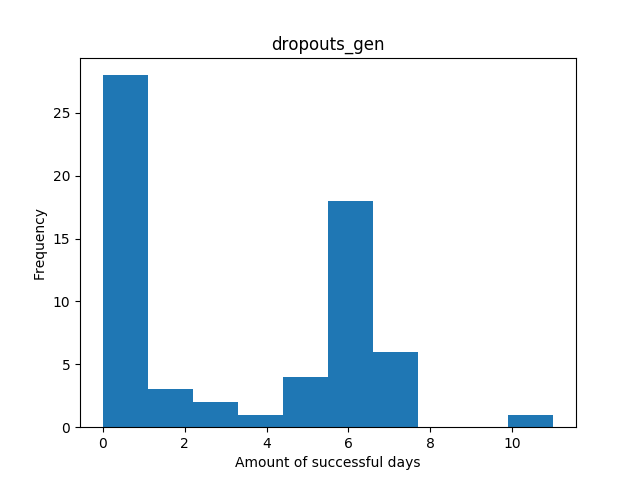
\includegraphics[width=.7\textwidth]{img/dropouts_gen.png}
    \caption{A histogram depicting the active days of all flashmap users}
    \label{fig:dropouts_gen}
\end{figure}
\begin{figure}
    \centering
    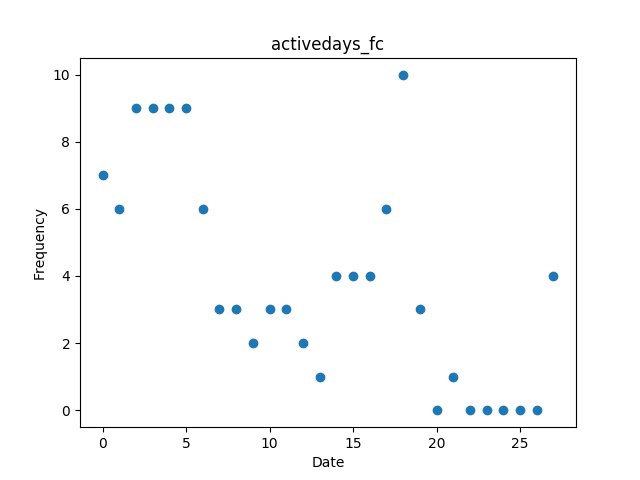
\includegraphics[width=.7\textwidth]{img/activedays_fc.png}
    \caption{A scatter diagram depicting how many flashcard users were active during which day of the experiment}
    \label{fig:activedays_fc}
\end{figure}
\begin{figure}
    \centering
    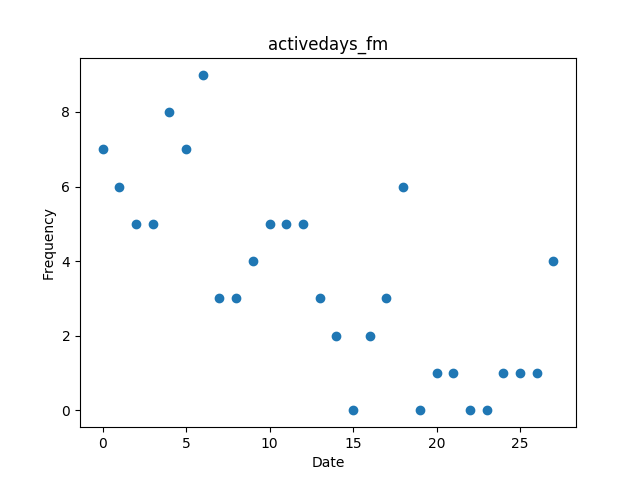
\includegraphics[width=.7\textwidth]{img/activedays_fm.png}
    \caption{A scatter diagram depicting how many flashmap users were active during which day of the experiment}
    \label{fig:activedays_fm}
\end{figure}
\begin{figure}
    \centering
    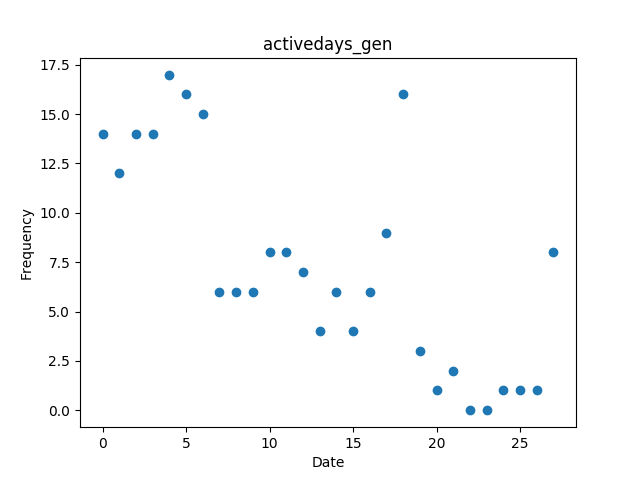
\includegraphics[width=.7\textwidth]{img/activedays_gen.png}
    \caption{A scatter diagram depicting how many users in total were active during which day of the experiment}
    \label{fig:activedays_gen}
\end{figure}

\section{Comparisons among conditions}

\begin{longtable}[c]{@{}lrrrr@{}}
\toprule\addlinespace
& \textbf{Mann-Whitney-U k} & \textbf{Mann-Whitney-U p} &
\textbf{Welch's t-test k} & \textbf{Welch's t-test p}
\\\addlinespace
\midrule\endhead
& 0.008 & 0.9936 & 0.008 & 0.9937
\\\addlinespace
\bottomrule
    \label{tab:dropouts-comp}
\end{longtable}

\begin{figure}[htbp]
    \centering
    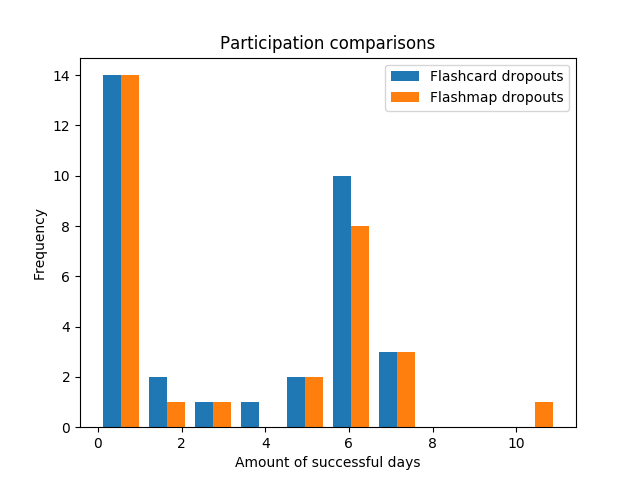
\includegraphics[width=.7\textwidth]{img/dropouts.png}
    \caption{A comparison of figure~\protect\ref{fig:dropouts_fc} and~\protect\ref{fig:dropouts_fm}}
    \label{fig:dropouts}
\end{figure}
